\section{Experiments}
\label{sec:expe}

In this part, we compare \Moca to other existing tools for memory analysis. In a first time, we present their main differences in terms of portability
and capabilities. Then, we present two sequences of quantitative experiments, one that outlines the importance of the default parameters chosen for our tool
and the other that compares the precision and performance of all the tools.

%\newpage

\subsection{Methodology}
\label{sec:exp-methodo}

%This section briefly discusses our experimental setup for the evaluation of
%\Moca.

Our main experiments were run on  machines from Grid5000 \Edel
cluster.
    As some state of the art tools can only run on AMD machines, we also ran
    some of the experiment presented in section~\ref{sec:expe-ovh} on
    \Stremi machine from Grid5000 grenoble.
    These machines hardware specifications
   \footnote{Grid5000 provides an online hardware description:\\
       \url{https://www.grid5000.fr/mediawiki/index.php/Grenoble:Hardware\#Edel}
       \\\url{https://www.grid5000.fr/mediawiki/index.php/Reims:Hardware\#Stremi}}
    are summarized in \tbl{hw}.

\begin{table}[t]
    \centering
    \begin{tabular}{lp{1.1cm}rrp{1.35cm}p{1.1cm}}
        \toprule
        \multirow{3}{.8cm}{CPU}
        %&  & \multicolumn{2}{c}{Vendor} & \multicolumn{2}{c}{Model} \\
        %\cmidrule(lr){3-6}
        & \Edel  & \multicolumn{4}{c}{Intel Xeon E5520} \\
        % & \Idfreeze & \multicolumn{2}{c}{AMD} & \multicolumn{2}{c}{Opteron 6174} \\
        & \Stremi & \multicolumn{4}{c}{AMD Opteron 6164 HE} \\
        \midrule
        \multirow{3}{.8cm}{System totals}
        & & Nodes & Threads & Freq & Memory \\
        \cmidrule(lr){3-6}
        & \Edel   & $2$ & $8$ & \SI{2.27}{Ghz} & \SI{24}{Gib} \\
        %& \Idfreeze & $8$ & $48$ & \SI{2.20}{Ghz} & \SI{256}{Gib}\\
        & \Stremi & $2$ & $24$ & \SI{1.7}{Ghz} & \SI{48}{Gib}\\
        \midrule
        \multirow{3}{.8cm}{Per node}
        & & Cores & Threads & L3 Cache & Memory \\
        \cmidrule(lr){3-6}
        & \Edel   & $4$ & $4$ & \SI{8}{Mib} & \SI{12}{Gib} \\
        %& \Idfreeze & $6$ & $6$  & \SI{12}{Mib} & \SI{32}{Gib} \\
        & \Stremi & $6$ & $6$  & \SI{12}{Mib} & \SI{24}{Gib} \\
        \bottomrule
    \end{tabular}
    \caption{Hardware configuration of our evaluation system.}
    \label{tab:hw}
\end{table}


\begin{table}[htb]
    \centering
    \begin{tabular}{lccccc}
        \toprule
        %& \multicolumn{5}{c}{Design} \\
        %\cmidrule{2-6}
        & \multicolumn{3}{c}{Mechanisms} & \multicolumn{2}{c}{Architecture} \\
        \cmidrule{2-6}
        \TABARNAC   & \multicolumn{3}{c}{Instrumentation}
        & \multicolumn{2}{c}{Intel, AMD} \\
        \Mitos      & \multicolumn{3}{c}{PEBS + Instrumentation}
        & \multicolumn{2}{c}{Intel} \\
        \MemProf    & \multicolumn{3}{c}{IBS}
        & \multicolumn{2}{c}{AMD} \\
        \Moca       & \multicolumn{3}{c}{Page faults (+Instrumentation)}
        & \multicolumn{2}{c}{\textbf{Any}}\\
        \midrule
        %& \multicolumn{5}{c}{Trace precision} \\
        %\cmidrule{2-6}
        & Granularity & Superset & Time &
        Thread sharing & CPU\\
        \cmidrule{2-6}
        \TABARNAC   & Page & \textbf{Page} & no & \textbf{yes} & no\\
        \Mitos      & \textbf{Address} & None  & \textbf{yes} & no & \textbf{yes}\\
        \MemProf    & \textbf{Address} & None & \textbf{yes} & \textbf{yes} & \textbf{yes}\\
        \Moca       & \textbf{Address} & \textbf{Page} & \textbf{yes} & \textbf{yes} & \textbf{yes}\\
        \bottomrule
    \end{tabular}
    \caption{Comparison of different memory traces tools.}
        \label{tab:tools-comp}
\end{table}

For each experiment, we deployed the same \emph{Debian} \emph{Jessie}
environment running a \texttt{Linux 3.16.0-4} on a machine with hyper threading
disabled. We disabled address space randomization to make the comparison between different
traces more practical. 
As our two evaluation machines do not have the same hardware,
we limited the number of threads used by openMP to $8$
that is the largest number of hardware threads available on both machines.


We evaluate \Moca by comparing it to the following state of the art tools. The first one,
\Mitos, is the tracing tool from MemAxes~\cite{Gimenez14Dissecting}.
%and relies on Intel PEBS technology.
The second one, \TABARNAC~\cite{Beniamine15TABARNACRR}, is one of our previous
contribution,
%It is based on a Pin instrumentation, which traps all the memory accesses but 
which only counts the number of time each thread accesses to each page.
%\DB{Is the following sentence useful ?}
%\GH{Pas vraiment}
%Although this is less precise than the information collected by \Moca, it does not require
%the management of large and complex data
%structures.
The third one, \MemProf~\cite{Lachaize12MemProf}, is designed to analyze NUMA
performance issues. %and relies on AMD IBS.
The main differences between \Moca and these other memory profiling tools are
summarized in \tbl{tools-comp}.

\begin{table}[htb]
    \centering
    \begin{tabular}{p{1.5cm}lcp{3.3cm}}
        \toprule
        Group & Name & Footprints* & Description \\
        \midrule
        \multirow{4}{1.5cm}{Memory Intensive}
        & \IS & \SI{132}{Mib} & Integer Sort \\
        & \CG & \si{125}{Mib} & Conjugate Gradient \\
        & \MG & \si{508}{Mib}& Multi-grid \\
        & \FT & \si{398}{Mib}& Discrete 3D FFT \\
        \midrule
        \multirow{2}{1.5cm}{Unstructured}
        & \UA & \si{112}{Mib}& Unstructured Adaptive mesh \\
        & \DC & $1.46$Gib & Data Cube \\
        \midrule
        \multirow{3}{1.5cm}{Pseudo Applications (solvers)}
        & \BT & \si{120}{Mib}& Block Tri-diagonal \\
        & \SP & \si{122}{Mib}& Scalar Penta-diagonal \\
        & \LU & \si{118}{Mib}& Lower-Upper Gauss-Seidel \\
        \midrule
        CPU bound & \EP & \si{78}{Mib}& Embarrassingly parallel \\
        \bottomrule
    \end{tabular}
    \caption{Description of the \NPB.\\
        *\emph{maximum memory used, measured with Valgrind}.}
    \label{tab:NPB}
\end{table}

In the following sections, all the tools are
evaluated on each of the 10 \NPB~\cite{Jin1999}, which are
presented in \tbl{NPB}, according to the information available on the nasa
website\footnote{\url{http://www.nas.nasa.gov/publications/npb.html}}.

Except for the experiment about the influence of \Moca's parameters, on each
experiment, \Moca has been run with it's default parameters: a wakeup interval of
\SI{0.5}{s} for the logging process and \SI{50}{ms} for the monitoring thread.
Each point in each plot is the average of at least $30$ executions. Along with each point,
the error bars represent the standard error.

We consider experimental reproducibility as an important matter, therefore we
distribute\footnote{See our experiment repository:
    \href{https://github.com/dbeniamine/Moca_expe}{github.com/dbeniamine/Moca\_expe}}
all the files needed to reproduce our experiments at three different levels:
The first level constains the filtered results (csv files) from the
experiments along with the \texttt{R-markdown} scripts that generated the
plots presented in this article.
% making possible the reproduction of our statistic analysis.
The second consists of the full raw traces generated by our experiments along
with the scripts used to extract the filtered traces (csv files from the
previous level) and the scripts used at the previous level to perform the
analysis.
Finally, at the most comprehensive level, we provide a git repository that
includes our deployment environment, dependencies to all the tools and files
required and instructions that explain how to reproduce the experiment with or
without access to grid5000.


%\subsection{Experiments}
\subsection{Moca default parameters}
\label{sec:expe-param}

Before comparing \Moca to existing tools, we need to evaluate the impact of
the wakeup intervals (logging daemon and monitor thread) on the trace
precision and on the overhead. To do so, we run the \IS benchmark instrumented by \Moca with
a wakeup interval ranging from \SI{0.1}{s} to  \SI{0.9}{s} for the logging daemon and from \SI{20}{ms} to
\SI{100}{ms} for the monitoring thread. For each run, we measure \IS execution time and the number of
accesses captured. We have chosen \IS for this evaluation as it is one of the memory intensive \NPB,
quick experiments with other ones confirmed these results. This experiment was
run on a machine from the \Edel cluster.

\begin{figure}[htb]
    \centering
    \begin{subfigure}{.9\linewidth}
        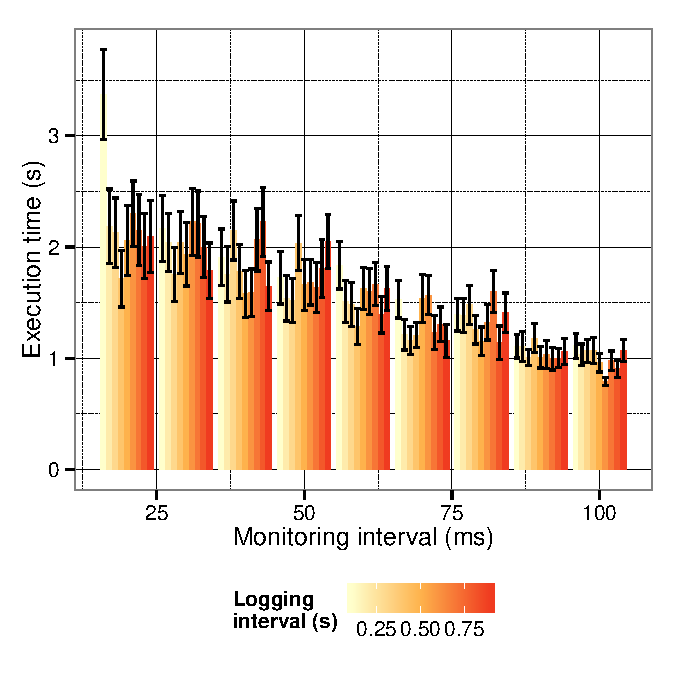
\includegraphics[width=\linewidth]{moca_param.pdf}
        \caption{Execution time.}
        \label{fig:param_time}
    \end{subfigure}
    \begin{subfigure}{.9\linewidth}
        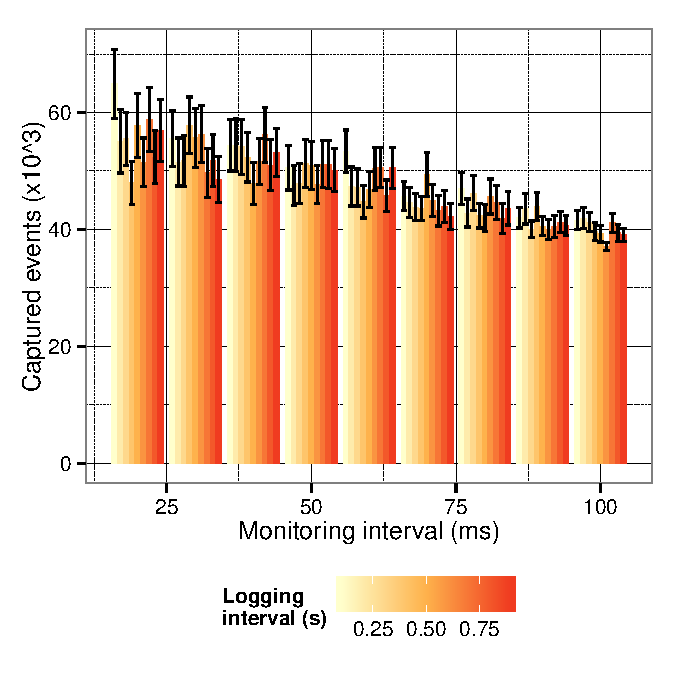
\includegraphics[width=\linewidth]{moca_param_events.pdf}
        \caption{Number of captured events.}
        \label{fig:param_evts}
    \end{subfigure}
    \caption{Influence of the wakeup intervals on \IS, class A.}
    \label{fig:param}
\end{figure}

We can see on the \fig{param_time} that the execution time increases when we
reduce the monitoring wakeup interval. At \SI{40}{ms}
it seems to reach its worst level, thus we should keep it larger. At \SI{50}{ms}, the default value we have chosen, the
\fig{param_evts} shows that we obtain more than two thirds of the events captured
at smaller intervals, which seems quite reasonable.
Regarding the logging interval, our experiments do not exhibit a clear trend. Changing it seems to interfere with the system I/Os scheduler resulting in chaotic
variations both in the execution time and the number of captured events. The fact that variations in execution time result in matching variations in the number
of captured events is due to the fixed length of monitoring intervals : the longer the execution, the more monitoring intervals there are and the more events
the trace contains. Overall these variations are not significant as all the confidence intervals intersect. 
Finally we have chosen a logging interval of \SI{0.5}{s}, the median value, in order to avoid unnoticed effect caused by extremum values.
\GH{Comment changer l'intervalle de logging peut-il avoir un impact sur le nombre d'évènements capturés ? Autre question un peu en
	lien : on a l'impression que les figures \fig{param_time} et \fig{param_evts} sont exactement les même à un niveau de zoom près. C'est possible mais un
peu étonnant si on tient compte de la question précédente}
\DB{Les courbes sont bien sortie sur des jeux de données différents. Je
    suppose que le temps d'execution et le nombre d'evenements sont très liés.
    Vu la taille des intervalles de conficance le “logging interval” n'influe
    pas beaucoup.
    Quoiqu'il en soit le fait de flusher la trace sur le disque déclenche pas
    mal d'I/O ce qui peut interferer avec l'appli observée et donc coup influer
    sur la qualité du sampling.}
\GH{Ok, ta dernière explication est plausible, mais ce qui est perturbant c'est qu'on ne voit pas de tendance : des fois on a plus d'évènement avec un petit
logging interval, d'autres fois non. Je rajoute une explication qui me paraît plausible et je te laisse voir}
%These two values have been chosen as default values in \Moca.


% \newpage

\subsection{Comparison with existing tools}
\label{sec:expe-ovh}

Preliminary experiments showed us that \Mitos capture by
default way less distinct pages than \TABARNAC and \Moca. Thus, we tried to change \Mitos
sampling period in order to make it capture at most pages as possible, 
we name this version \MitosTun. Surprisingly, its behavior regarding this sampling period
is not monotonous, we had to try many different periods to find the proper one.

The default \MemProf distribution did not work with our experimental setup. With the help
of their support team\footnote{see issue at
    \href{https://github.com/Memprof/scripts/issues/1}{github.com/Memprof/scripts/issues/1}}, we managed to make it work by disabling the library used to retrieve
data structures names. For the same reason as in the case of \Mitos, our study includes
two version of \MemProf: the default version and \MemProfTun for which we have
increased the sampling rate to its maximum.

Finally our evaluation also differentiate \Moca (kernel module only) from
\MocaPin which also retrieve the data structure information using a Pin
instrumentation, we make this distinction to evaluate the impact of Pin on
\Moca performances.

We compare the different tools on two aspects: trace precision and induced slowdown. Regarding the trace precision, the first experiment compares the tools
using two criteria:  the
percentage of captured pages and the number of captured events.  We use \TABARNAC as a reference to compute the total number of pages accessed by the
application because, by design, it traps all the memory accesses to compute the number performed in each page. This metric is representative of coverage of the
memory space: the capacity of the tool to outline the whole memory area accessed by the application. Regarding the number of captured events, we present the percentage
relative to \Moca, as it is the tool that usually provides the more precise traces. We define one event as one
timestamped access found in the trace file outputted by a tool. According to this definition, \TABARNAC does not capture any events as it only keep one
counter per page and per thread without any temporal informations. Thus, \TABARNAC is excluded from this comparison. The number of captured events is representative
of the precision of a monitoring tool, its capacity to keep track of all the evolutions of the access patterns during the course of the execution. The idea is
that, the more the tool captures events, the less it misses changes in the access patterns.

The second experiment compares the
slowdown factor of the different tools.  All these experiments have been run on each of the \NPB on class A.

\begin{figure}[htb]
    \centering
    \begin{subfigure}{\linewidth}
        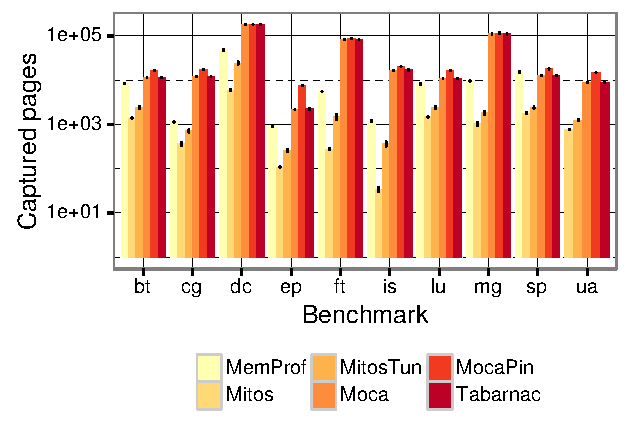
\includegraphics[width=\linewidth]{moca_pages_intel.pdf}
        \caption{Percentage of captured pages.}
        \label{fig:pages}
    \end{subfigure}
    \begin{subfigure}{\linewidth}
        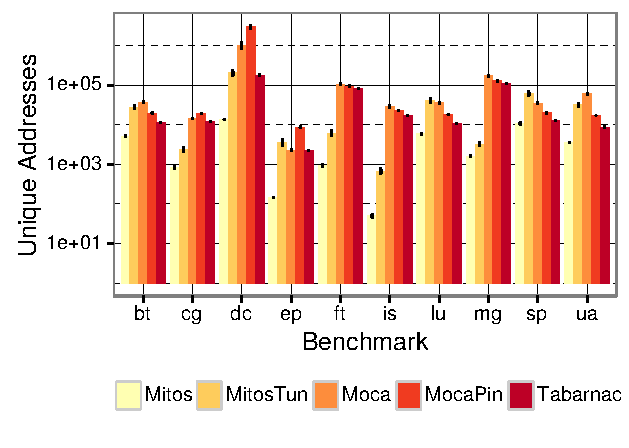
\includegraphics[width=\linewidth]{moca_addr_intel.pdf}
        \caption{Percentages of events captured (compared to \Moca).}
        \label{fig:addr}
    \end{subfigure}
    \caption{Precision of the traces generated by each tool.}
    \label{fig:pages-addr}
\end{figure}

\fig{pages-addr} presents the results of the precision evaluation of the
different tools. The values used for \Mitos, \MitosTun, \Moca and
\TABARNAC result from runs on \Edel machines, while \MemProf and \MemProfTun values result from runs on
\Stremi.

We can see on \fig{pages} that \Moca captures almost as many pages as \TABARNAC.
Regarding their design they should capture as many pages. Nevertheless, there is a slight
bump in the number of pages used by applications monitored by \TABARNAC due to the Pin instrumentation.
Indeed, its JIT instrumentation recompiles the executable on the fly and changes the memory footprint
(of the stack, mainly). Thus, we can safely ignore these differences.
%and take \Moca as reference. \GH{Incohérent avec le choix précédent de prendre tabarnac comme référence}

\Mitos usually collect less than \SI{12.5}{\%} of the pages, adding some fine tunning
can almost double this number but it still misses most of the address space.

Concerning \MemProf, changing the default sampling rate does not seems to
have any noticeable impact on the end result. Both \MemProf and \MemProfTun captures significantly more pages than
\Mitos and \MitosTun. Nevertheless, for half of the studied applications it does
not see more than \SI{50}{\%} of the addresses space. Only for, \BT, \LU, \SP and \UA,
\MemProf manages to capture around \SI{75}{\%} of the accessed pages. This is explained by the fact that all these
benchmarks are using uniformly most of their address space, and that many pages are frequently accessed.
This is coherent with the fact that \MemProf is solely based on instructions sampling and only sees the most accesses pages.

From \fig{addr} we can see that, as expected, for almost every benchmarks,
\Moca collects significantly more events than the other tools.  The only
benchmark for which \Moca is not the more precise tool is \EP which is an
Embarrassingly Parallel application with very few memory accesses.
This outlines the fact that \Moca captures events in an uniform way, timed by the monitoring interval.
On the contrary, the other tools might capture more events in a few hotspots presents in the application but miss
sparse accesses during the rest of the execution.
For almost
every other benchmarks both \Mitos (with or without tunning) and \MemProf
hardly reach \SI{10}{\%} of the accesses collected by \Moca, the only exception is
\DC for which \MemProf captures from \SI{25}{\%} to \SI{50}{\%} of the accesses
collected by \Moca.
%\GH{Je ne vois pas ça sur la figure, erreur ?} Erreur CG au lieu de DC

These results prove that most existing tools can miss a considerable part of
the address-space while \Moca guarantee that it provides a superset of the accessed
pages. Furthermore they show that \Moca is the only existing tool able to provide a
trace that is precise enough to give an good overview of the memory behavior of an application. In
short, not only our tool provides a complete trace at the granularity of the
page but it is also significantly more precise than the other existing tools.

\begin{figure}[htb]
    \centering
    \begin{subfigure}{\linewidth}
        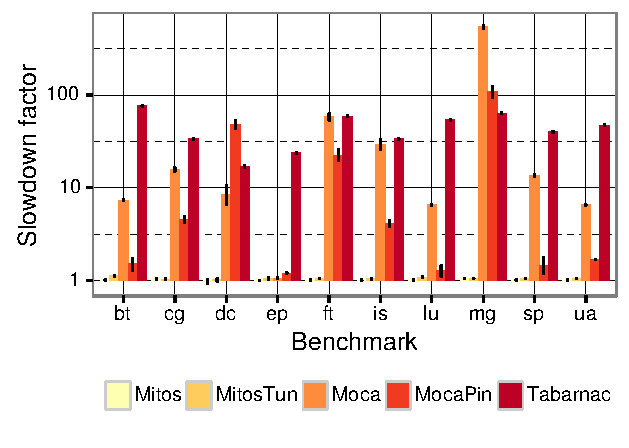
\includegraphics[width=\linewidth]{moca_overhead_intel.pdf}
        \caption{Evaluation on \Edel (Intel)}
        \label{fig:ovh-Intel}
    \end{subfigure}
    \begin{subfigure}{\linewidth}
        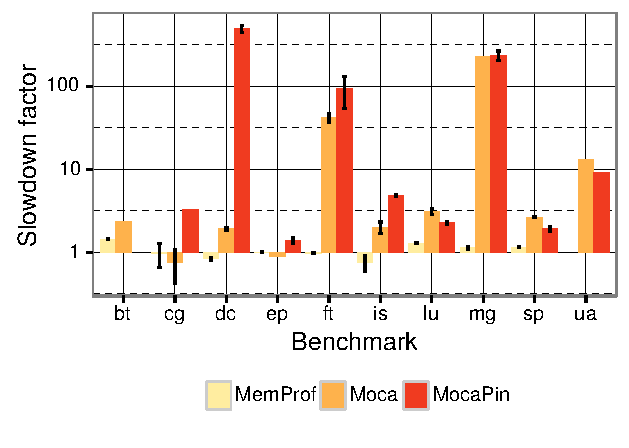
\includegraphics[width=\linewidth]{moca_overhead_amd.pdf}
        \caption{Evaluation on \Stremi (AMD)}
        \label{fig:ovh-AMD}
    \end{subfigure}
    \caption{Slowdown factor of each tool.
    Y-axis in log scale.}
    \label{fig:ovh}
\end{figure}

\fig{ovh} shows for each of the \NPB, the slowdown factor when
instrumented by \Moca and the other existing tools on Intel
(\fig{ovh-Intel}) and AMD (\fig{ovh-AMD}) Machines. Notice that the Y-axis is in
log scale.

From \fig{ovh-Intel}, we can see that \Mitos, \MitosTun overhead is
almost negligible which is not the case for \Moca and \TABARNAC, this
difference is explained by the results of the previous experiment, as these
tools usually collects less than \SI{10}{\%} of the accesses collected by \Moca and
miss a significant part of the address space.

We can classify the benchmarks into three groups:
for \BT, \CG, \DC,  \EP, \LU, \SP and \UA, \Moca is
significantly faster than \TABARNAC. This set of benchmarks is interesting as
it is made of varied application profiles as we can see in \tbl{NPB}.
Indeed, if \EP is mostly doing parallel computation with only a few number of
memory accesses, \CG is described as memory intensive,
\BT, \LU as well as \SP are linear algebra solvers with regular memory access patterns,
and both \UA and \DC contain \emph{unstructured computation,
parallel I/O and data movement}. Furthermore, \DC has a considerable memory footprint as
described in \tbl{NPB}.
%\GH{Ce n'est pas ce que je vois dans la table : UA semble comme les autres et le chiffre pour DC, 146Gib me paraît énorme, erreur ?}
% Le 146 etait du a \SI qui mangait le '.' \ldots
% UA et DC sont unstructured, effectivement UA n'a pas une grosse emprunt
% mémoire \ldots

The second group only contains memory intensive benchmarks (\FT and
\IS). For this group, \Moca is as good as \TABARNAC or a bit faster, probably
because the balance between computations and memory accesses hides the
overhead of the instrumentation.
%\GH{Dans les deux paragraphes précédents il y a les termes memory intensive, significant usage of memory et memory oriented. Les perfs sont différentes mais ces
%trois termes semblent dire la même chose, ... on se demande du coup... }
%\DB{J'ai reformulé un peu, mais ces courbes montrent que mêmes des bench dites
%memory intensive peuvent avoir des performances correctes avec Moca}

For the last benchmark: \MG, \Moca is significantly slower than \TABARNAC.
%It is important to note that \MG is not the benchmark using the largest set of addresses, 
%therefore, the poor performance likely comes from a thread scheduling issue rather than from the size of the benchmark.
\GH{Ca, pour moi, ça sort du chapeau. Tu as un argument ? Moi je dirais plutôt qu'il balai largement son espace mémoire (même petit)
durant toute son exécution}
\DB{J'ai mal exprimé mon idée, en gros je pensait a un ordo bien pourrit du
    point de vu de Moca (en gros qui déclenche plein de prise de verrous),
    mais ça semble effectivement capilotracté.
Ton argument est plus raisonnable}
\GH{J'ai réécrit, je te laisse voir.}
By looking at our
experiment logs, we found that \MG generates a lot of conflicts in the hash map used by
\Moca to store false page faults. This issue is caused by applications that perform a very large number of sparse accesses to a large working set.
This is not usual as parallel applications are often optimized to make memory accesses as local as possible in order to take advantage of all the levels of the
memory hierarchy.
Thus, we consider this benchmark as a pathological case.
A solution could be to increase the size of
this hash map, which is not always possible as memory space in the kernel is
limited (and these experiments have been run with the largest hash map we could use). Another easier solution would consist in working on a smaller instance
of \MG and see if the trace is still useful. Although the results are not presented here, we have run \Moca on \MG with a smaller size (W) and we have been able
to confirm that the performance becomes comparable to \TABARNAC in this case.
\GH{On a des résultats avec MG plus petit ?}

\fig{ovh-AMD} shows the results of the evaluation on the AMD machine
(\Stremi). On this machine, \Moca overhead is quite similar to the one
obtained on \Edel.
\MemProf exhibits a slowdown factor comparable to \Mitos while
providing traces a little more precise. Nevertheless, they are still \emph{incomplete} and
way less precise than \Moca traces. Obviously \MemProfTun has the same
overhead than \MemProf as it capture the same amount of data.

Finally, we can see, as expected, that adding one execution with a Pin
instrumentation to retrieve data structures information (\MocaPin) only adds a small overhead
to the whole \Moca execution. For several benchmarks this difference is so small that we cannot
distinguish it from \Moca usual overhead.

%\subsection{Summary}
%\label{sec:expe-cncl}

%We have tested \Moca with various applications and using several parameters.
%Our experiments, show that \Moca has a good behavior for a wide range of
%parameters and helped us defining their default values. Our experiments also
%show that, with these parameters, \Moca provides significantly more precise traces
%than state of the art tools.
%Of course, because of this increased precision, \Moca is slower than two of these tools,
%\MemProf and \Mitos.
%Nevertheless, the comparison with \TABARNAC outlines the fact that, when a superset of the memory
%space is captured, \Moca efficiency is good.
%Doing this using \MemProf and \Mitos, and provide the same guarantee, would require to sample all the memory instructions, which is not possible.
%At the end of the day, \Moca is the only tool able to provide a
%detailed trace with temporal, spacial and sharing information while providing
%guarantees on the information lost during the sampling.
